%\renewcommand{\theequation}{\theenumi}
%\begin{enumerate}[label=\arabic*.,ref=\thesubsection.\theenumi]
%\numberwithin{equation}{enumi}
%

\item Show that the points $\vec{A} = \myvec{1\\7}, \vec{B} = \myvec{4\\2}, \vec{C}=\myvec{-1\\-1},\vec{D}= \myvec{-4\\4} $  are the vertices of a square.
\\
\solution By inspection, 
%
\begin{align}
\frac{\vec{A}+\vec{C}}{2}=\frac{\vec{B}+\vec{D}}{2} = \myvec{0\\3}
\end{align}
%
Hence, the diagonals $AC$ and $BD$ bisect each other.
%
Also, 
\begin{align}
\brak{\vec{A}-\vec{C}}^T
\brak{\vec{B}-\vec{D}} = 0
\end{align}
%
$\implies AC \perp BD $.  Hence $ABCD$ is a square.
\item If the points
$
\vec{A} = \myvec{6\\1}, 
\vec{B} = \myvec{8\\2}, 
\vec{C} = \myvec{9\\4}, 
\vec{D} = \myvec{p\\3}
$
are the vertices of a parallelogram, taken in order, find the value of $p$.
\\
\solution In the parallelogram $ABCD$, $AC$ and $BD$ bisect each other.  This can be used to find $p$.
\item If $\vec{A} = \myvec{-5\\7}, \vec{B} = \myvec{-4\\-5}, \vec{C} = \myvec{-1\\-6}, \vec{D} = \myvec{4\\5}$, find the area of the quadrilateral $ABCD$.
%
\\
\solution The area of  $ABCD$ is the sum of the areas of trianges ABD and CBD and is given by 
\begin{multline}
\frac{1}{2}\norm{\brak{\vec{A}-\vec{B}}\times \brak{\vec{A}-\vec{D}}}
\\
+
\frac{1}{2}\norm{\brak{\vec{C}-\vec{B}}\times \brak{\vec{C}-\vec{D}}}
\end{multline}
\item Show that the points 
$\vec{A} = \myvec{1\\2\\3},
 \vec{B} = \myvec{-1\\-2\\-1},
\vec{C} = \myvec{2\\3\\2},
\vec{D} = \myvec{4\\7\\6}.
$
are the vertices of a parallelogram $ABCD$ but it is not a rectangle.
%
\\
\solution Since the direction vectors
%
\begin{align}
\vec{A}-\vec{B}&= \vec{D}-\vec{C}
\\
\vec{A}-\vec{D}&= \vec{B}-\vec{C}
\end{align}
%
$AB \parallel CD$ and $AD \parallel BC$.  Hence $ABCD$ is a parallelogram.  However, 
%
\begin{align}
\brak{\vec{A}-\vec{B}}^T\brak{ \vec{A}-\vec{D}}\ne 0
\end{align}
%
Hence, it is not a rectangle.
The following code plots Fig. \ref{fig:quad_3d}
%
\begin{lstlisting}
codes/triangle/quad_3d.py
\end{lstlisting}
%
\begin{figure}[!ht]
\includegraphics[width=\columnwidth]{./triangle/figs/quad_3d.eps}
\caption{}
\label{fig:quad_3d}
\end{figure}
%

\item Find the area of a parallelogram whose adjacent sides are given by the vectors \myvec{3\\1\\4} and \myvec{1\\-1\\1}.
%
\\
\solution  The area is given by 
%
\begin{align}
\frac{1}{2}\norm{\myvec{3\\1\\4} \times \myvec{1\\-1\\1}}
\end{align}
%
\item $ABCD$ is a rectangle formed by the points $\vec{A} = \myvec{-1\\-1}, \vec{B} = \myvec{-1\\4}, \vec{C} = \myvec{5\\4}, \vec{D} = \myvec{5\\-1}$. $ \vec{P}, \vec{Q}, \vec{R}, \vec{S}$ are the mid points of $AB, BC, CD, DA$ respectively.  Is the quadrilateral $PQRS$ a 
\begin{enumerate}
\item square?
\item rectangle?
\item rhombus?
\end{enumerate}
\solution
\input{./solutions/quad/1/solution}
\item $ABCD$ is a cyclic quadrilateral with 
\begin{align}
\angle A &= 4y+20
\\
\angle B &= 3y-5
\\
\angle C &= -4x
\\
\angle D &= -7x+5
\end{align}
%
Find its angles.
\\
\solution
\input{./solutions/2/chapters/quadilateral_ex/solution.tex}
\item Draw a quadrilateral in the Cartesian plane, whose vertices are \myvec{– 4\\ 5}, \myvec{0\\ 7}, \myvec{5\\ – 5} and \myvec{– 4\\ –2}. Also, find its area.
\\
\solution
\input{./solutions/3/chapters/quad/solution.tex}

\item Find the area of a rhombus if its vertices are 
\begin{align}
\vec{P} &= \myvec{3\\0}, \vec{Q} =\myvec{4\\5},
\\
\vec{R} &= \myvec{-1\\4}, \vec{S} = \myvec{-2\\-1} 
\end{align}
taken in order.
\\
\solution
\input{./solutions/4/chapters/quadrilateral/solution.tex}
\item Without using distance formula, show that points \myvec{– 2\\ – 1}, \myvec{4\\ 0}, \myvec{3\\ 3} and \myvec{–3\\ 2} are the vertices of a parallelogram.
\\
\solution
\input{./solutions/5/chapters/quadrilateral/docq4.tex}
\item  Find the area of the quadrilateral whose vertices, taken in order, are 
 \myvec{-4\\2},  \myvec{-3\\-5},  \myvec{3\\-2},  \myvec{2\\3}. 
\\
\solution
\input{./solutions/6/chapters/quadrilateral/solution.tex}
\item The two opposite vertices of a square are \myvec{-1\\2},  \myvec{3\\2}. Find the coordinates of the other two vertices.
\\
\solution
\input{./solutions/7/chapters/quad/solution1.tex}
\item Find the area of a parallelogram whose adjacent sides are given by the vectors \myvec{3\\1\\4} and \myvec{1\\-1\\1}.
\\
\solution
\input{./solutions/quad/8/chapters/solution.tex}
\item Find the area of a rectangle $ABCD$ with vertices
$\vec{A} = \myvec{-1\\\frac{1}{2}\\ 4},
 \vec{B} = \myvec{1\\\frac{1}{2}\\ 4},
\vec{C} = \myvec{1\\-\frac{1}{2}\\ 4},
\vec{D} = \myvec{-1\\-\frac{1}{2}\\ 4}.
$
\\
\solution
\input{./solutions/quad/10/solution.tex}
\item The two adjacent sides of a parallelogram are \myvec{2\\ -4 \\ -5} and  \myvec{1\\-2\\ -3}. Find the unit vector parallel to its diagonal.  Also, find its area.
%
\\
\solution

 Let 
    \begin{align}
        \vec{A}=\myvec{2\\-4\\-5}, \vec{B}=\myvec{1\\-2\\-3}
    \end{align}
    be the adjacent sides of the parallelogram. Let $\vec{D}$ be the diagonal of the parallelogram. Then,
    \begin{align}
        \vec{D}&=\vec{A}+\vec{B}\\
&=\myvec{3\\-6\\-8}
    \end{align}
   \begin{align}
       \norm{\vec{D}}=\sqrt{(3)^2+(-6)^2+(-8)^2}=\sqrt{109}
   \end{align}
   Let $\vec{U}$ be the unit vector of $\vec{D}$ which can be found as follows:
   \begin{align}
       \vec{U}=\frac{\vec{D}}{\norm{\vec{D}}}
   \end{align}
   Solving the above equation gives the unit vector $\vec{U}$ which is parallel to the diagonal $\vec{D}$.\\
   \begin{align}\therefore
       \boxed
       {\vec{U}=\frac{1}{\sqrt{109}}\myvec{3\\-6\\-8}}
   \end{align}
  %   \begin{align}
%        \norm{\vec{A}\times\vec{B}}
%    \end{align}
%    where
   \begin{align}
  \because     \vec{A}\times\vec{B} &=\myvec{0&-A_3&A_2\\A_3&0&-A_1\\-A_2&A_1&0}\myvec{B_1\\B_2\\B3}\\
       &=\myvec{0&5&-4\\-5&0&-2\\4&2&0}\myvec{1\\-2\\-3}=\myvec{2\\1\\0},
       \\
       \norm{\vec{A}\times\vec{B}}&=\sqrt{(-2)^2+(1)^2+(0)^2}\\
       &=\sqrt{5}
\end{align}
which is the desired area.  
% \centering
% 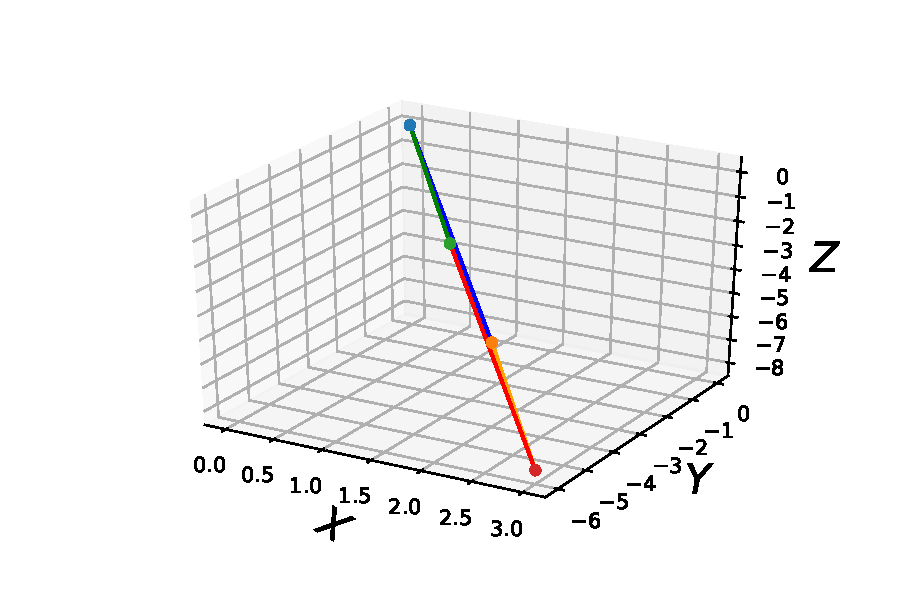
\includegraphics[width=\columnwidth]{solutions/july/1/Figures/parallelogram.pdf}
% \caption{}
% \label{Fig 1.2}
% \end{figure}



%\end{enumerate}
%
